\documentclass[11pt]{article}

\usepackage[margin=0.78in]{geometry}
\usepackage{graphicx}
\usepackage{booktabs}
\usepackage{longtable}
\usepackage{array}
\usepackage[dvipsnames]{xcolor}
\usepackage{hyperref}
\usepackage{enumitem}
\usepackage{float}
\usepackage{listings}
\usepackage{caption}
\usepackage{url}
\usepackage{amsmath}
\usepackage{amssymb}

\graphicspath{{../assets/screenshots/}}
\hypersetup{
  colorlinks=true,
  linkcolor=MidnightBlue,
  urlcolor=MidnightBlue,
  citecolor=MidnightBlue
}

\definecolor{ink}{HTML}{101820}
\definecolor{coral}{HTML}{CC6048}
\definecolor{teal}{HTML}{226F68}
\definecolor{amber}{HTML}{C9952E}
\definecolor{bone}{HTML}{FFF8EA}
\definecolor{slate}{HTML}{253238}
\definecolor{softgray}{HTML}{F4EFE6}

\lstdefinestyle{code}{
  basicstyle=\ttfamily\small,
  breaklines=true,
  frame=single,
  rulecolor=\color{softgray},
  backgroundcolor=\color{softgray},
  keywordstyle=\color{teal}\bfseries,
  commentstyle=\color{coral},
  stringstyle=\color{amber},
  showstringspaces=false
}
\lstset{style=code}

\newcommand{\product}{ReliaGuard Studio}
\newcommand{\model}{ReliaGuard-NS}
\newcommand{\codepath}[1]{\nolinkurl{#1}}
\newcommand{\cmd}[1]{\texttt{\detokenize{#1}}}
\newcommand{\state}[1]{\textbf{#1}}

\setlength{\parskip}{0.55em}
\setlength{\parindent}{0pt}
\renewcommand{\arraystretch}{1.15}
\sloppy

\title{\vspace{-1.5em}\textbf{\product}\\Complete Project Explanation}
\author{Ahan Bhatt}
\date{\today}

\begin{document}

\maketitle

\begin{center}
\fcolorbox{teal}{bone}{
  \begin{minipage}{0.92\linewidth}
  \textbf{One-sentence summary.} \product{} is a production-style AI reliance observability platform. Teams can upload historical human-AI logs, stream live decision events through SDKs, call a guardrail API during assisted decisions, review flagged cases, tune thresholds, and generate reliance audits for overreliance, underreliance, calibration, and unsafe decision behavior.
  \end{minipage}
}
\end{center}

\tableofcontents
\newpage

\section{What The Project Is}

\product{} is a productized AI evaluation platform. It is not just a research script collection and it is not a clinical or diagnostic system. The project studies a specific product-safety question:

\begin{quote}
Can an AI system improve average performance while still creating harmful decision behavior in individual human-AI interactions?
\end{quote}

The answer is yes. A user might:

\begin{itemize}[leftmargin=*]
  \item accept wrong AI advice even though their original answer was correct;
  \item reject correct AI advice even though their original answer was wrong;
  \item become poorly calibrated after seeing AI output;
  \item require an uncertainty cue or evidence-comparison prompt before finalizing;
  \item appear successful on average while still showing dangerous reliance failures.
\end{itemize}

\product{} turns those hidden patterns into concrete product outputs:

\begin{itemize}[leftmargin=*]
  \item bring-your-own-log audits;
  \item Python and TypeScript SDK event streaming;
  \item live guardrail actions such as allow, request verification, show uncertainty, delay, and route to review;
  \item project workspaces;
  \item review queues and reviewer labels;
  \item reliance-state probabilities;
  \item calibrated harmful-reliance risk;
  \item uncertainty estimates;
  \item symbolic rule traces;
  \item counterfactual suggestions;
  \item conformal thresholds;
  \item selective-gating actions;
  \item model-evaluation, replay, monitoring, and policy-simulation dashboards.
\end{itemize}

The current public-data evidence layer integrates 43,263 records from 2,229 participants or students across five public datasets: HAIID, CHI 2023 DKE, ConvXAI, Pardos/Bhandari ChatGPT tutoring, and FLoRA IPS. The app and API turn that research framing into a portfolio-ready, production-style platform.

\section{Screenshots And User Experience}

\subsection{Homepage}

The landing page explains the product in under 30 seconds. It leads with the thesis that average accuracy is insufficient and then shows the five-dataset evidence base, product outputs, and navigation to the simulator and dashboards.

\begin{figure}[H]
  \centering
  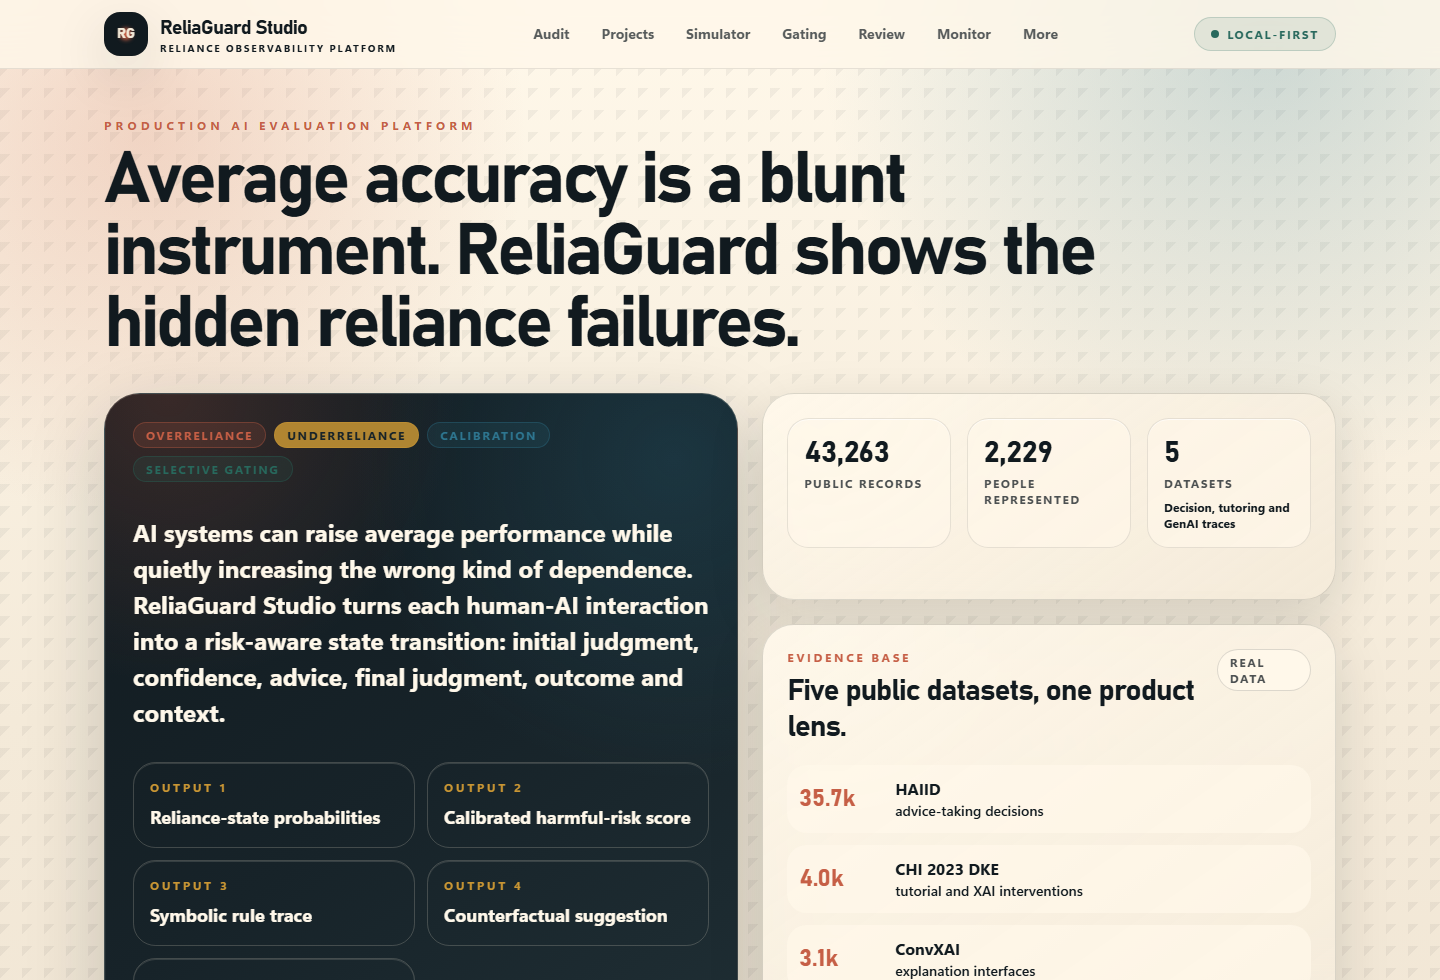
\includegraphics[width=\linewidth]{01-homepage.png}
  \caption{ReliaGuard Studio homepage. The hero section frames the product around hidden reliance failures and shows the main outputs: state probabilities, calibrated risk, symbolic rule traces, counterfactual suggestions, and selective-gating actions.}
\end{figure}

\subsection{Interactive Case Simulator}

The simulator is the centerpiece of the app. It lets a user enter one human-AI decision tuple and receive a full reliance trace.

\begin{figure}[H]
  \centering
  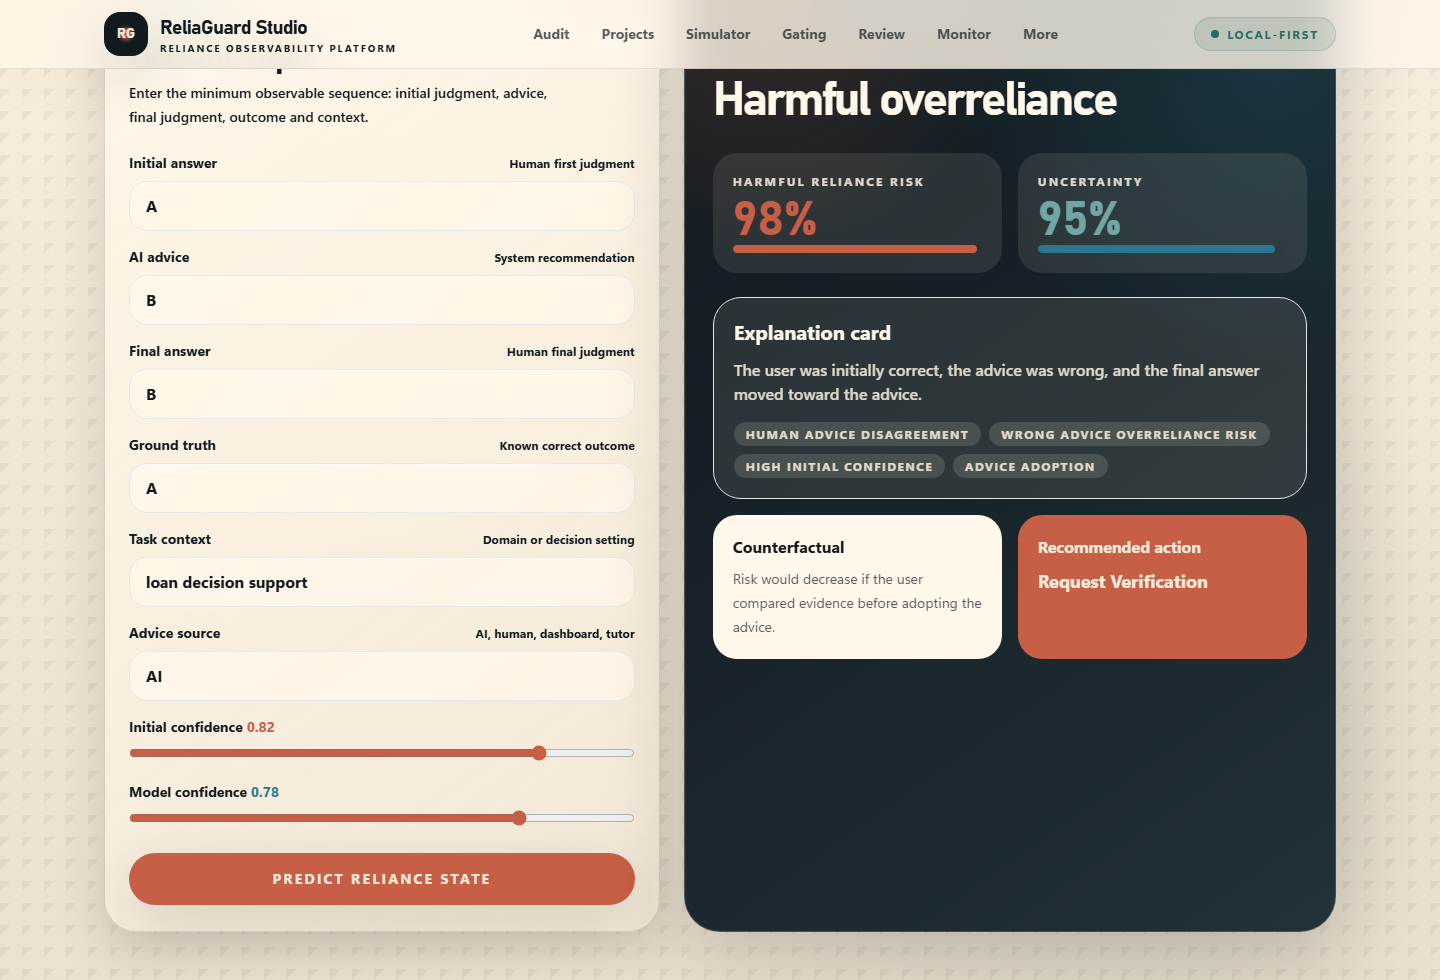
\includegraphics[width=\linewidth]{02-simulator-result.png}
  \caption{Interactive simulator result. The example shows harmful overreliance: the human was initially correct, the advice was wrong, and the final answer moved toward the wrong advice.}
\end{figure}

\subsection{Conformal Gating Dashboard}

The gating dashboard lets a user vary the allowed harmful-case miss rate, denoted by alpha. Lower alpha asks the system to miss fewer harmful cases, which usually increases intervention burden.

\begin{figure}[H]
  \centering
  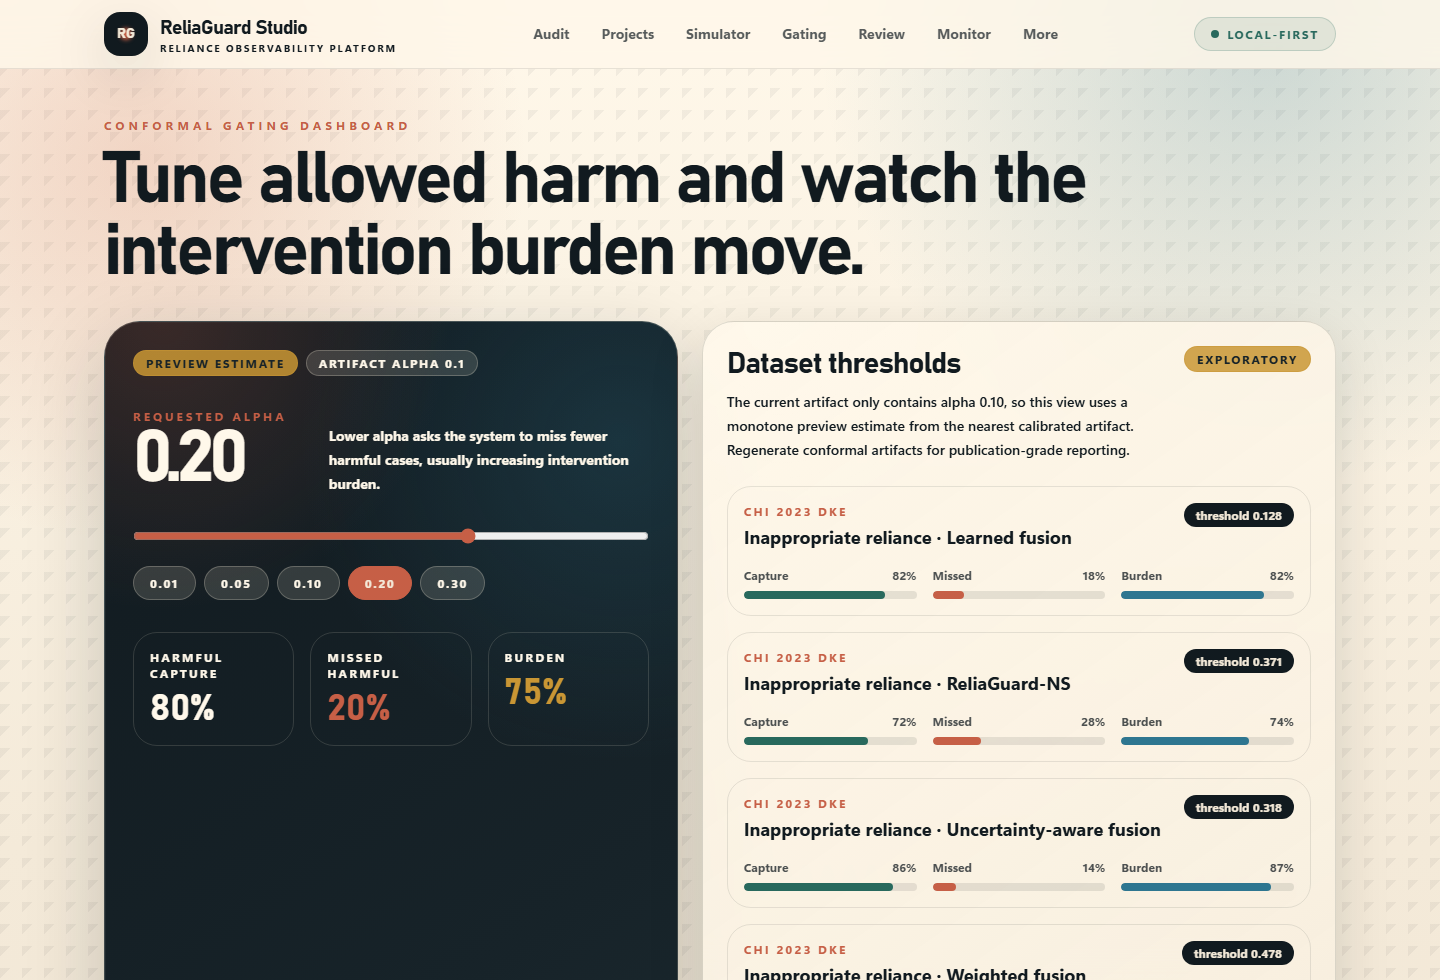
\includegraphics[width=\linewidth]{03-gating-dashboard.png}
  \caption{Conformal gating dashboard. The alpha slider exposes the trade-off between harmful-case capture, missed harmful cases, and intervention burden. Preview rows are labelled as exploratory when exact calibrated artifacts are not available for the requested alpha.}
\end{figure}

\subsection{Model Evaluation Lab}

The evaluation lab makes model performance, calibration, and split rigor visible rather than hiding them behind a single aggregate metric.

\begin{figure}[H]
  \centering
  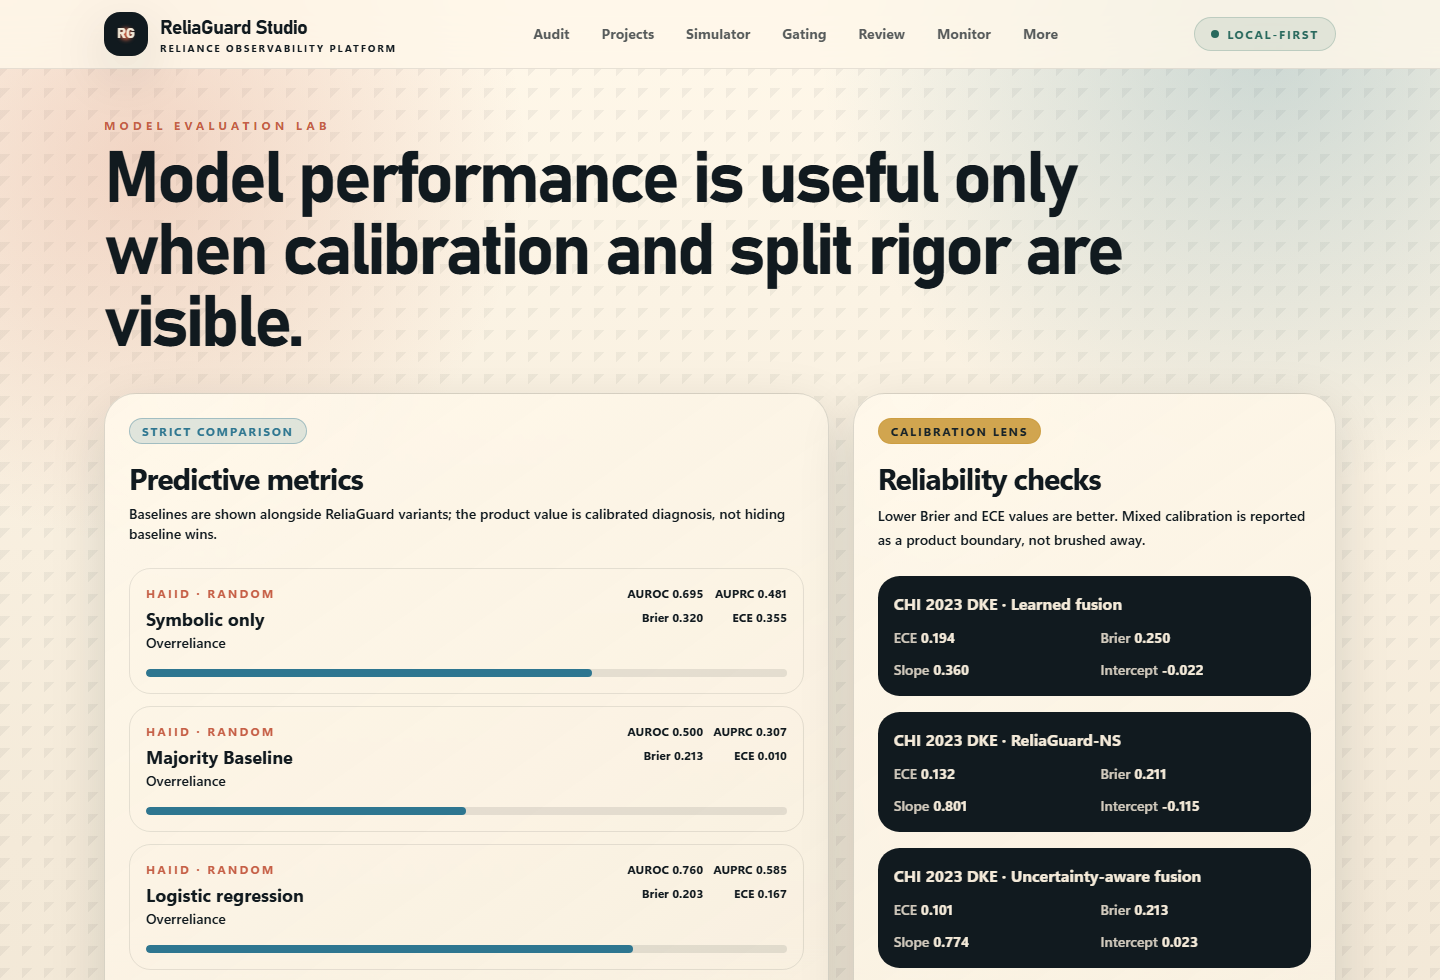
\includegraphics[width=\linewidth]{04-evaluation-lab.png}
  \caption{Model evaluation lab. The dashboard shows predictive metrics and calibration checks so that model quality is evaluated beyond accuracy alone.}
\end{figure}

\subsection{Upload Logs Audit}

The upload workflow turns \product{} from a demo into a usable observability product. A team can upload CSV, JSON, or JSONL logs, map their own columns into the canonical ReliaGuard schema, validate missing fields, and generate an audit report with state distributions and highest-risk cases.

\begin{figure}[H]
  \centering
  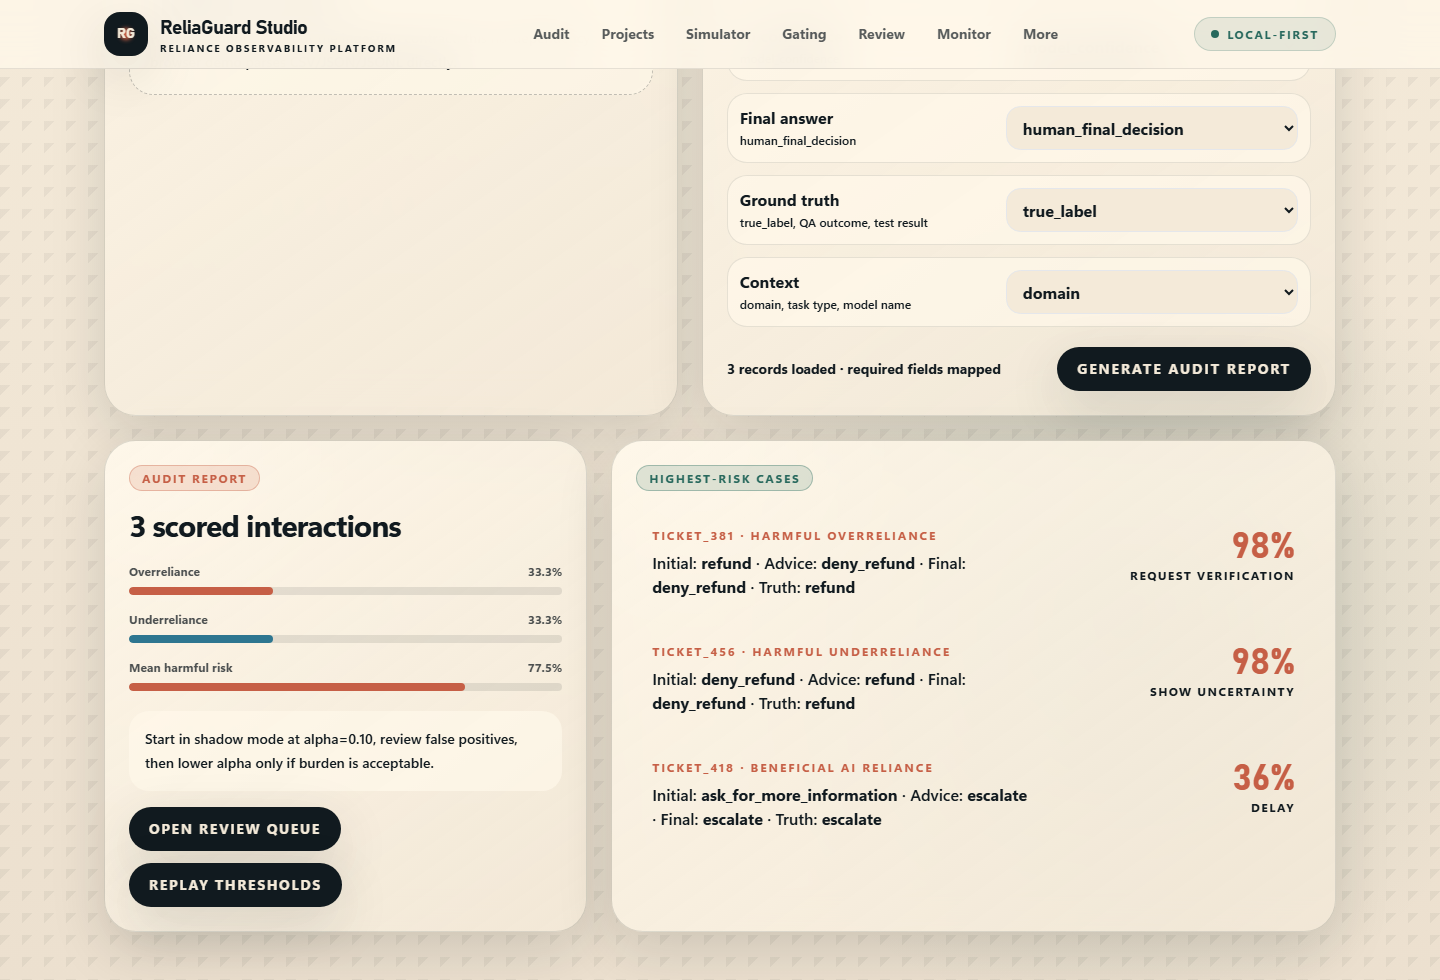
\includegraphics[width=\linewidth]{05-upload-audit.png}
  \caption{Upload logs audit report. The page maps user columns to ReliaGuard fields, scores the uploaded customer-support demo records, and summarizes overreliance, underreliance, mean harmful risk, and highest-risk cases.}
\end{figure}

\subsection{Review Queue}

The review queue closes the product feedback loop. Flagged cases can be labelled as true harmful reliance, false positive, uncertain, bad ground truth, intervention worked, or intervention too burdensome. These labels help teams tune thresholds and understand intervention burden before deployment.

\begin{figure}[H]
  \centering
  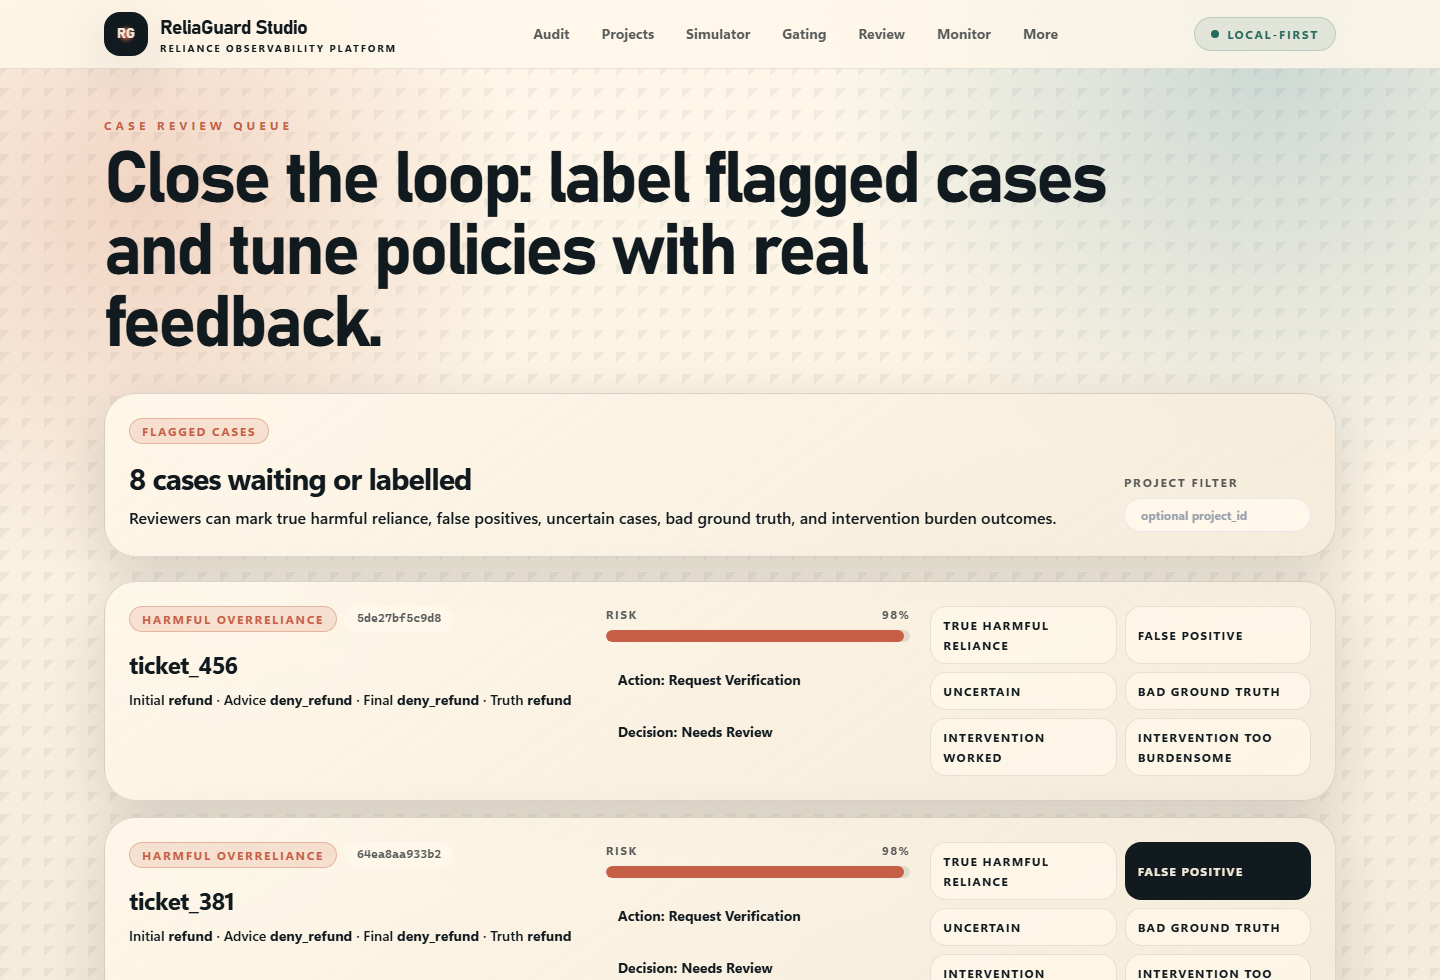
\includegraphics[width=\linewidth]{06-review-queue.png}
  \caption{Review queue. Flagged cases are sorted by risk and paired with reviewer labels so product teams can audit false positives, ground-truth problems, and intervention burden.}
\end{figure}

\subsection{Monitoring}

The monitoring page is the production observability view. It summarizes streamed and uploaded events by reliance state, recommended action, reviewer feedback, and context risk.

\begin{figure}[H]
  \centering
  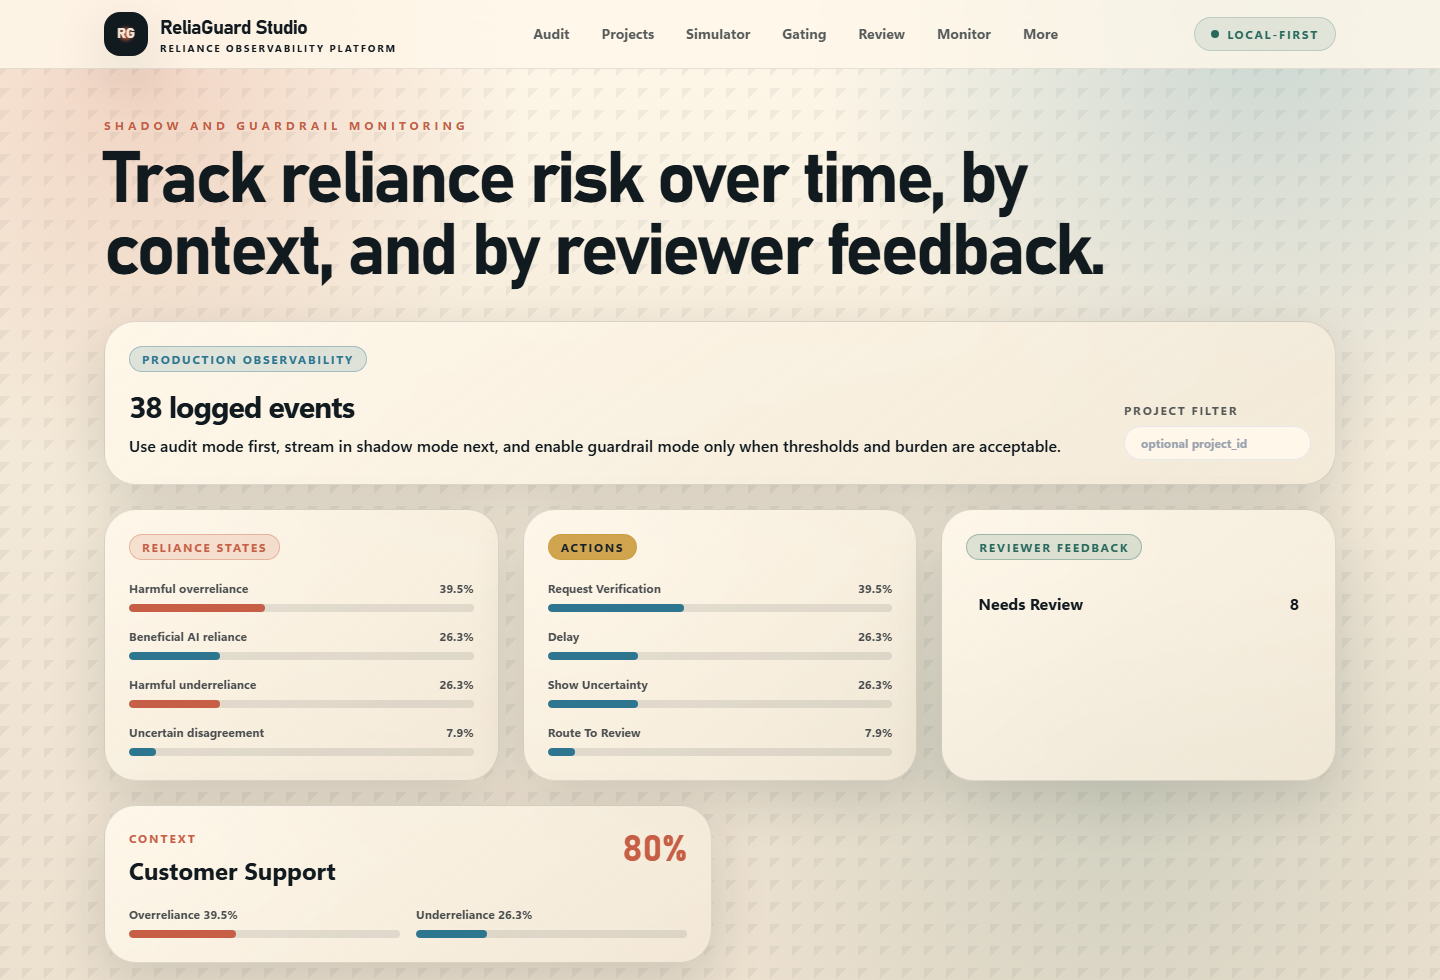
\includegraphics[width=\linewidth]{07-monitoring.png}
  \caption{Monitoring dashboard. ReliaGuard tracks logged events, reliance-state rates, action distribution, reviewer feedback, and risk by context.}
\end{figure}

\section{Repository Structure}

The repository is organized as a full-stack product and research software package:

\begin{longtable}{p{0.28\linewidth} p{0.66\linewidth}}
\toprule
\textbf{Path} & \textbf{Purpose} \\
\midrule
\codepath{apps/web/} & Next.js, TypeScript, Tailwind frontend. It contains the product UI: homepage, upload logs, projects, simulator, gating dashboard, review queue, monitoring, replay, interventions, evaluation lab, policy page, data page, guide, and limitations page. \\
\codepath{apps/api/} & FastAPI product entrypoint. This wraps the main Python API and exposes endpoints for prediction, explanation, thresholds, datasets, policy simulation, ablation, and model-card metadata. \\
\codepath{packages/relia\_core/} & Product-facing wrapper package. It provides a cleaner import boundary for downstream services while the core logic remains in the main Python package. \\
\codepath{sdks/python/} & Installable Python SDK for logging human-AI interactions and calling live guardrail checks from external systems. \\
\codepath{sdks/typescript/} & TypeScript SDK for browser or server-side AI applications that need event streaming or guardrail actions. \\
\codepath{src/reliaguard\_studio/} & Main installable Python package. It contains data adapters, schemas, models, rules, statistics, visualization helpers, API logic, study scaffold, and CLI commands. \\
\codepath{src/reliaguard\_studio/api/} & FastAPI application and product output schemas. \\
\codepath{src/reliaguard\_studio/data/} & Data loading, canonical schemas, dataset screening, storage, simulation utilities, and public-dataset adapters. \\
\codepath{src/reliaguard\_studio/models/} & Baselines, fusion methods, reliance-state model, sequence model scaffolds, and \model{} components. \\
\codepath{src/reliaguard\_studio/rules/} & Fuzzy and symbolic rule engine for reliance-state explanations and rule bundles. \\
\codepath{src/reliaguard\_studio/evaluation/} & Metrics, calibration, GEE statistics, policy evaluation, conformal risk control, sensitivity analysis, leakage audits, and cross-dataset analysis. \\
\codepath{src/reliaguard\_studio/visualization/} & Figure generation, SVG utilities, visual identity, contact sheets, render-safety checks, and table generation helpers. \\
\codepath{src/reliaguard\_studio/study\_platform/} & Prospective validation scaffold for future human-subject studies. It includes tasks, randomization, quality checks, data schema, exports, reports, and simulations. \\
\codepath{src/reliaguard\_studio/theory/} & Formal reliance-state definitions and utility-bound helpers. \\
\codepath{docs/} & Public documentation: architecture, deployment, usage, schema guides, guardrail API docs, integration notes, model cards, portfolio text, screenshots, sample logs, and this PDF source. \\
\codepath{infra/} & Docker Compose and deployment scaffolding. \\
\codepath{tests/} & Unit, integration, product API, statistics, model, rule, and smoke tests. \\
\codepath{artifacts/} & Ignored generated data, prepared tables, model outputs, runtime databases, and experiment outputs. \\
\codepath{paper/} & Ignored manuscript and paper artifacts. Kept out of public GitHub publication. \\
\codepath{.private/} & Ignored local-only material such as legacy files, audits, and unpublished review materials. \\
\bottomrule
\end{longtable}

\section{Full-Stack Architecture}

The product is split into a web client, API service, and Python intelligence layer.

\subsection{Frontend}

The frontend lives in \codepath{apps/web}. It is built with Next.js, TypeScript, Tailwind, and a custom visual style. The key pages are:

\begin{longtable}{p{0.25\linewidth} p{0.67\linewidth}}
\toprule
\textbf{Page} & \textbf{Role} \\
\midrule
\codepath{/} & Landing page. Presents the problem, evidence scale, product outputs, and navigation. \\
\codepath{/upload} & Bring-your-own-data workflow. Upload CSV/JSON/JSONL logs, map columns, validate fields, generate audit summaries, and create review-queue cases. \\
\codepath{/projects} & Project workspace view for saved thresholds, policies, model versions, reviewer notes, reports, and exports. \\
\codepath{/simulator} & Interactive single-case simulator. Sends a decision tuple to the backend and renders state, risk, uncertainty, rule trace, counterfactual, and action recommendation. \\
\codepath{/gating} & Conformal gating dashboard. Lets the user vary alpha and inspect harmful capture, missed harmful cases, and intervention burden. \\
\codepath{/review} & Case review queue for labelled feedback on harmful reliance, false positives, bad ground truth, and intervention burden. \\
\codepath{/monitoring} & Shadow and guardrail monitoring view. Summarizes reliance states, actions, reviewer feedback, and risk by context. \\
\codepath{/replay} & Historical replay view for estimating what different threshold or policy choices would have flagged. \\
\codepath{/interventions} & Intervention template library that maps risk patterns to concrete product prompts and routing actions. \\
\codepath{/evaluation} & Model evaluation lab. Displays predictive metrics, calibration checks, and split-rigor framing. \\
\codepath{/policy} & Policy simulation page. Compares intervention policies such as no gating, confidence thresholds, symbolic gating, and \model{} gating. \\
\codepath{/data} & Data and reproducibility page. Explains public datasets and pipeline commands. \\
\codepath{/guide} & User guide for setup and project interpretation. \\
\codepath{/limitations} & Safety and evidence-boundary page. \\
\bottomrule
\end{longtable}

The frontend never reads raw datasets directly. It calls the FastAPI backend through typed helpers in \codepath{apps/web/lib/api.ts}.

\subsection{Backend}

The backend entrypoint is \codepath{apps/api/main.py}, which imports the FastAPI app from \codepath{src/reliaguard\_studio/api/main.py}. The API exposes product endpoints over JSON.

\begin{longtable}{p{0.36\linewidth} p{0.56\linewidth}}
\toprule
\textbf{Endpoint} & \textbf{Output} \\
\midrule
\codepath{GET /model-card} & Intended use, limitations, datasets, outputs, and non-use cases. \\
\codepath{GET /datasets} & Public dataset summary. \\
\codepath{POST /predict-reliance} & Reliance state, harmful risk, uncertainty, state probabilities, active rules, counterfactual, action, explanation, and safety boundary. \\
\codepath{POST /explain-case} & Plain-language explanation, active rules, counterfactual, recommended action, and constrained assistant-style response. \\
\codepath{GET /conformal-threshold?alpha=...} & Dataset/model threshold rows for selective risk control. \\
\codepath{GET /simulate-policy} & Offline policy-simulation outputs. \\
\codepath{GET /run-ablation} & Rule/model ablation outputs if artifacts are present. \\
\codepath{GET /evaluation-lab} & Model metrics, calibration rows, and cross-dataset transfer summaries. \\
\codepath{GET /v1/projects} & Project workspaces with modes, thresholds, policies, model versions, notes, and report history. \\
\codepath{POST /v1/events/log} & SDK event logging endpoint for completed human-AI interactions. \\
\codepath{POST /v1/guardrail/check} & Live guardrail endpoint that returns allow, request verification, show uncertainty, delay, or route to review. \\
\codepath{POST /v1/ingest/validate} & Bring-your-own-log ingestion endpoint that validates mapped records and generates an audit report. \\
\codepath{GET /v1/review-queue} & Flagged cases for human reviewer feedback. \\
\codepath{POST /v1/replay} & Historical replay endpoint for threshold and policy what-if analysis. \\
\codepath{GET /v1/monitoring} & Monitoring summary for streamed and uploaded events. \\
\codepath{GET /v1/interventions} & Intervention template library. \\
\codepath{GET /api/health} & Basic service health. \\
\bottomrule
\end{longtable}

\subsection{Core Python Package}

The core package is \codepath{src/reliaguard\_studio}. This is the source of truth for:

\begin{itemize}[leftmargin=*]
  \item configuration loading and validation;
  \item public dataset adapters;
  \item reliance-state definitions;
  \item symbolic and fuzzy rule logic;
  \item baseline and fusion models;
  \item conformal thresholding;
  \item calibration metrics;
  \item policy simulation;
  \item claims and leakage audits;
  \item figure and table generation;
  \item CLI commands.
\end{itemize}

\section{How External Teams Plug In}

\product{} supports three deployment stages.

\subsection{Audit Mode: Upload Historical Logs}

A team can upload historical AI-assisted decision logs, map their columns into ReliaGuard fields, and generate an audit report. The canonical fields are:

\begin{longtable}{p{0.30\linewidth} p{0.58\linewidth}}
\toprule
\textbf{ReliaGuard Field} & \textbf{Common Source Columns} \\
\midrule
\codepath{user\_id} & \codepath{agent\_id}, \codepath{learner\_id}, \codepath{reviewer\_id} \\
\codepath{task\_id} & \codepath{ticket\_id}, \codepath{question\_id}, \codepath{case\_id} \\
\codepath{initial\_answer} & \codepath{human\_first\_decision} \\
\codepath{initial\_confidence} & \codepath{confidence\_before\_ai} \\
\codepath{ai\_advice} & \codepath{model\_recommendation} \\
\codepath{ai\_confidence} & \codepath{model\_confidence} \\
\codepath{final\_answer} & \codepath{human\_final\_decision} \\
\codepath{ground\_truth} & \codepath{true\_label}, QA outcome, test result \\
\codepath{context} & domain, task type, model name \\
\bottomrule
\end{longtable}

\subsection{Shadow Mode: Stream Events}

In shadow mode, a product streams completed decisions to ReliaGuard without interrupting users. The Python SDK exposes:

\begin{lstlisting}[language=Python]
from reliaguard import ReliaGuard

rg = ReliaGuard(api_key="local-dev")
rg.log_interaction(
    project_id="support-copilot",
    user_id="agent_123",
    task_id="ticket_456",
    initial_answer="refund",
    initial_confidence=0.72,
    ai_advice="deny_refund",
    ai_confidence=0.88,
    final_answer="deny_refund",
    ground_truth="refund",
    context={"domain": "customer_support"}
)
\end{lstlisting}

\subsection{Guardrail Mode: Call During A Decision}

In guardrail mode, a host application calls \codepath{POST /v1/guardrail/check}. The response contains a state, risk, uncertainty, active rules, message, and recommended action. If ground truth is unavailable during a live decision, ReliaGuard returns proxy risk and an uncertainty boundary rather than pretending it knows the confirmed reliance state.

\section{How The Simulator Works In Detail}

The simulator is a concrete product interface over the reliance-state model. It answers:

\begin{quote}
Given what the human thought first, what advice they saw, what they chose finally, and what was actually correct, what kind of reliance behavior occurred?
\end{quote}

\subsection{Input Tuple}

The simulator input can be written as:

\[
x = (h_0, c_0, a, h_1, y, d, s, m)
\]

where:

\begin{longtable}{p{0.18\linewidth} p{0.72\linewidth}}
\toprule
\textbf{Symbol} & \textbf{Meaning} \\
\midrule
$h_0$ & Human initial answer before seeing advice. \\
$c_0$ & Human initial confidence. \\
$a$ & AI or support-system advice. \\
$h_1$ & Human final answer after seeing advice. \\
$y$ & Ground truth or known correct answer. \\
$d$ & Task context or domain. \\
$s$ & Advice source, such as AI, human, dashboard, or tutor. \\
$m$ & Model confidence or reliability signal attached to the advice. \\
\bottomrule
\end{longtable}

\subsection{Derived Behavioral Signals}

The backend computes:

\begin{align*}
\text{initial\_correct} &= \mathbb{1}[h_0 = y] \\
\text{advice\_correct} &= \mathbb{1}[a = y] \\
\text{final\_correct} &= \mathbb{1}[h_1 = y] \\
\text{disagreement} &= \mathbb{1}[h_0 \ne a] \\
\text{adopted\_advice} &= \mathbb{1}[h_1 = a]
\end{align*}

These are deliberately simple. The point is not to hide the model behind an opaque neural score. The point is to turn observable interaction logs into interpretable reliance-state evidence.

\subsection{State Definitions}

\begin{longtable}{p{0.30\linewidth} p{0.60\linewidth}}
\toprule
\textbf{Reliance State} & \textbf{Conservative Definition} \\
\midrule
\state{Beneficial AI reliance} & The human was initially wrong, advice was correct, and the final answer adopted the correct advice. \\
\state{Harmful overreliance} & The human was initially correct, advice was wrong, and the final answer adopted the wrong advice. \\
\state{Harmful underreliance} & The human was initially wrong, advice was correct, and the final answer failed to adopt correct advice. \\
\state{Correct self-reliance} & The human was initially correct, advice was wrong, and the final answer stayed correct. \\
\state{Independent correct} & The final answer was correct without a sharper advice-dependence pattern. \\
\state{Independent incorrect} & The final answer was wrong without a sharper advice-dependence pattern. \\
\state{Uncertain disagreement} & The available tuple shows disagreement but does not support a stronger label. \\
\bottomrule
\end{longtable}

For example, the README screenshot uses:

\begin{lstlisting}
initial_answer = "A"
ai_advice      = "B"
final_answer   = "B"
ground_truth   = "A"
\end{lstlisting}

Because the human was initially correct, advice was wrong, and the final answer adopted advice, the state is \state{harmful overreliance}.

\subsection{Risk, Uncertainty, Rules, And Action}

After the state is identified, the product API returns a richer object:

\begin{lstlisting}[language=Python]
{
  "state": "harmful_overreliance",
  "harmful_reliance_risk": 0.98,
  "uncertainty": 0.95,
  "state_probabilities": {...},
  "active_rules": [
    "human_advice_disagreement",
    "wrong_advice_overreliance_risk",
    "high_initial_confidence",
    "advice_adoption"
  ],
  "counterfactual": "Risk would decrease if the user compared evidence before adopting the advice.",
  "recommended_action": "request_verification"
}
\end{lstlisting}

The harmful-risk score is bounded between 0 and 1 and is influenced by state, disagreement, confidence, and advice pressure. The uncertainty score increases when human confidence and model confidence are far apart. The active rules make the decision auditable, and the counterfactual translates the trace into a product recommendation.

\section{Data Layer}

\subsection{Datasets}

The public pipeline is built around five evidence sources:

\begin{longtable}{p{0.24\linewidth} p{0.18\linewidth} p{0.46\linewidth}}
\toprule
\textbf{Dataset} & \textbf{Scale} & \textbf{Main Construct Support} \\
\midrule
HAIID & about 35.7k interactions & Initial answer, advice, final answer, advice source, advice correctness, overreliance, underreliance, advice uptake, task-family heterogeneity. \\
CHI 2023 DKE & about 4.0k records & Intervention and XAI conditions, self-assessment calibration, appropriate reliance and inappropriate reliance. \\
ConvXAI & about 3.1k records & Explanation interfaces, conversational XAI conditions, confidence/reliability signals, appropriate reliance and overreliance. \\
Pardos/Bhandari & 274 learners & Short-term learning gains under no help, human-authored help, and ChatGPT-generated help. \\
FLoRA IPS & 275 students & GenAI-assisted process traces, writing/log behavior, prompt/process features, final proposal scores. \\
\bottomrule
\end{longtable}

\subsection{Canonical Schema}

The data adapters map heterogeneous files into canonical concepts:

\begin{itemize}[leftmargin=*]
  \item dataset name;
  \item participant or student identifier;
  \item task or item identifier;
  \item initial response;
  \item final response;
  \item advice value;
  \item advice source;
  \item ground truth;
  \item confidence before and after advice, if available;
  \item correctness before and after advice;
  \item advice correctness;
  \item movement toward advice;
  \item movement away from advice;
  \item overreliance;
  \item underreliance;
  \item appropriate reliance;
  \item learning gain or process outcome when relevant.
\end{itemize}

Raw and prepared data are written under ignored artifact directories so public GitHub publication does not redistribute participant-level data.

\section{Model Layer}

\subsection{Baselines}

The modeling stack includes ordinary baselines because the project must show that the neuro-symbolic layer is not being compared only against weak methods. Baselines include:

\begin{itemize}[leftmargin=*]
  \item majority and heuristic baselines;
  \item logistic regression;
  \item calibrated logistic regression;
  \item random forest;
  \item histogram gradient boosting;
  \item calibrated gradient boosting;
  \item MLP baselines where appropriate.
\end{itemize}

\subsection{Symbolic Models}

The symbolic model encodes domain-specific reliance logic. Rule groups include:

\begin{itemize}[leftmargin=*]
  \item wrong-advice overreliance;
  \item correct-advice underreliance;
  \item high-confidence vulnerability;
  \item correct self-reliance under disagreement;
  \item confidence inflation;
  \item low metacognitive prompting;
  \item high copy/paste or low source-engagement process signals when process data is available.
\end{itemize}

Rules produce both scores and explanation traces.

\subsection{Fusion And ReliaGuard-NS}

\model{} combines:

\begin{itemize}[leftmargin=*]
  \item tabular model estimates;
  \item symbolic rule activations;
  \item uncertainty estimates;
  \item reliance-state probabilities;
  \item conformal thresholds;
  \item selective-gating policies.
\end{itemize}

The project does not claim a universal raw-prediction breakthrough. Its product value is calibrated diagnosis: turning a model score into an auditable failure mode and a cautious intervention recommendation.

\section{Conformal Gating}

Conformal gating controls a score-based intervention policy. The user chooses an alpha value, which represents the tolerated harmful-case miss rate in the calibrated score distribution. Lower alpha means the product should miss fewer harmful cases, but usually intervenes more often.

\begin{longtable}{p{0.24\linewidth} p{0.66\linewidth}}
\toprule
\textbf{Quantity} & \textbf{Meaning} \\
\midrule
Alpha & Allowed harmful-case miss rate target for the score-control view. \\
Threshold & Score cutoff above which ReliaGuard recommends intervention. \\
Harmful capture & Fraction of harmful cases caught by the intervention rule. \\
Missed harmful & Fraction of harmful cases not caught. \\
Intervention burden & Fraction of all cases receiving an intervention. \\
Non-intervention coverage & Fraction of cases allowed through without intervention. \\
\bottomrule
\end{longtable}

The dashboard labels preview rows when exact calibrated artifacts do not exist for a requested alpha. This is important: UI exploration is not presented as a fresh scientific guarantee.

\section{Policy Simulation}

The policy page compares intervention strategies:

\begin{itemize}[leftmargin=*]
  \item no gating;
  \item confidence-threshold gating;
  \item symbolic-rule gating;
  \item \model{} conformal gating.
\end{itemize}

Policy simulation is observational. It estimates utility trade-offs using existing data and assumptions; it does not prove that showing a warning will causally change human behavior. A prospective randomized study would be required for that claim.

\section{Evaluation And Statistics}

The evaluation layer is designed around reviewer-grade checks:

\begin{itemize}[leftmargin=*]
  \item AUROC, AUPRC, F1, balanced accuracy;
  \item Brier score and expected calibration error;
  \item calibration slope/intercept;
  \item reliability summaries;
  \item random split, participant split, task/domain split, and cross-dataset transfer;
  \item GEE with participant clustering where repeated observations exist;
  \item bootstrap confidence intervals;
  \item sensitivity to label definitions and confidence thresholds;
  \item leakage checks;
  \item negative controls;
  \item rule and feature ablations;
  \item policy-burden sensitivity.
\end{itemize}

The project carefully distinguishes:

\begin{longtable}{p{0.22\linewidth} p{0.68\linewidth}}
\toprule
\textbf{Term} & \textbf{Meaning In This Project} \\
\midrule
Measurement & Mapping observable interaction traces to reliance-state labels. \\
Prediction & Estimating future or held-out reliance behavior under validation splits. \\
Explanation & Describing why a case was flagged through symbolic rules and counterfactuals. \\
Policy simulation & Observational utility analysis of candidate intervention policies. \\
Causal intervention & Not claimed without future prospective randomized validation. \\
\bottomrule
\end{longtable}

\section{Command-Line Interface}

The CLI command is \codepath{nsca}. It is defined in \codepath{pyproject.toml} and points to \codepath{reliaguard\_studio.cli:app}.

\begin{longtable}{p{0.36\linewidth} p{0.54\linewidth}}
\toprule
\textbf{Command} & \textbf{Purpose} \\
\midrule
\cmd{nsca search-datasets} & Show the dataset registry and screening decisions. \\
\cmd{nsca download-real-data} & Download public datasets into ignored artifacts. \\
\cmd{nsca prepare-real-data} & Build canonical prepared tables. \\
\cmd{nsca run-real-experiments} & Run primary public-data analyses. \\
\cmd{nsca run-cross-dataset} & Run cross-dataset construct transfer tests. \\
\cmd{nsca run-policy-evaluation} & Run offline policy simulation. \\
\cmd{nsca run-conformal-risk-control} & Compute conformal selective-risk rows. \\
\cmd{nsca generate-real-figures} & Generate real-data figures when paper artifacts are enabled locally. \\
\cmd{nsca audit-figures} & Run figure quality checks. \\
\cmd{nsca audit-render-safety} & Check that rendering avoids unsafe browser behavior. \\
\cmd{nsca audit-visual-text} & Scan visual outputs for bad labels. \\
\cmd{nsca audit-claims} & Audit manuscript or report claims where artifacts are available. \\
\cmd{nsca build-paper} & Build the private paper package when local ignored files exist. \\
\cmd{nsca serve-api} & Run the API service. \\
\cmd{nsca run-all} & Run the public pipeline sequence. \\
\bottomrule
\end{longtable}

\section{How To Run The App}

\subsection{One-Command Windows Launcher}

The easiest way to run the app locally is:

\begin{lstlisting}[language=bash]
.\run_app.ps1
\end{lstlisting}

The script checks dependencies, starts the FastAPI backend, starts the Next.js frontend, prints the API and web URLs, and keeps both services alive until interrupted.

\subsection{Manual Backend}

\begin{lstlisting}[language=bash]
python -m pip install -e ".[dev]"
uvicorn apps.api.main:app --reload --host 127.0.0.1 --port 8000
\end{lstlisting}

\subsection{Manual Frontend}

\begin{lstlisting}[language=bash]
cd apps/web
npm install
npm run dev
\end{lstlisting}

\subsection{Docker Compose}

\begin{lstlisting}[language=bash]
docker compose -f infra/docker-compose.yml up --build
\end{lstlisting}

\section{Testing And Quality Gates}

The key checks are:

\begin{lstlisting}[language=bash]
pytest
python -m compileall src tests
cd apps/web
npm run typecheck
npm run build
\end{lstlisting}

The tests cover configuration loading, metrics, models, rules, end-to-end API behavior, product API endpoints, policy/statistics utilities, negative controls, prospective-study scaffolds, leakage audits, and real-data pipeline behavior.

\section{Screenshot Generation}

README screenshots are generated from the live app using a headless Chromium workflow:

\begin{lstlisting}[language=bash]
cd apps/web
npm install
npx playwright install chromium
cd ../..
node scripts/capture_readme_screenshots.mjs
\end{lstlisting}

The script starts the API and web app, captures the homepage, simulator result, gating dashboard, evaluation lab, upload-audit workflow, review queue, and monitoring dashboard, writes images under \codepath{docs/assets/screenshots/}, and shuts down only the spawned processes.

\section{Publication And Privacy Safety}

The project is meant to be public as a product/code repository while protecting unpublished research paper content. The following paths are ignored:

\begin{itemize}[leftmargin=*]
  \item \codepath{paper/}
  \item \codepath{artifacts/}
  \item \codepath{.private/}
  \item \codepath{CLAIMS\_CHECKLIST.md}
  \item local build caches;
  \item node modules;
  \item Python caches and egg-info.
\end{itemize}

Before pushing, run:

\begin{lstlisting}[language=bash]
git status --ignored
git check-ignore -v paper artifacts .private CLAIMS_CHECKLIST.md
\end{lstlisting}

\section{Evidence Boundaries And Non-Claims}

\product{} is intentionally conservative. It supports:

\begin{itemize}[leftmargin=*]
  \item decision reliance;
  \item overreliance;
  \item underreliance;
  \item correct self-reliance;
  \item confidence and calibration signals;
  \item short-term tutoring learning-gain analysis;
  \item observational GenAI process-trace analysis;
  \item model calibration and split robustness;
  \item non-causal policy simulation.
\end{itemize}

It does not support:

\begin{itemize}[leftmargin=*]
  \item clinical diagnosis;
  \item cognitive decline claims;
  \item delayed recall claims;
  \item transfer-learning claims unless future data supports them;
  \item long-term learning claims;
  \item causal claims that warnings change deployed human behavior without a prospective randomized study.
\end{itemize}

\section{How The Pieces Fit Together}

The complete flow is:

\begin{enumerate}[leftmargin=*]
  \item Public datasets are downloaded or staged into ignored artifact folders.
  \item Data adapters map dataset-specific columns into canonical reliance concepts.
  \item The evaluation pipeline builds descriptive statistics, labels, model metrics, calibration summaries, and policy artifacts.
  \item The Python package exposes the core scoring functions and API models.
  \item FastAPI serves product endpoints for the frontend.
  \item The Next.js frontend renders the homepage, simulator, gating dashboard, evaluation lab, policy page, data page, guide, and limitations page.
  \item The simulator converts a single decision tuple into a reliance state, risk, uncertainty, rules, counterfactual, and recommended action.
  \item The gating dashboard turns calibrated score artifacts into a selectable intervention-burden view.
  \item The evaluation lab makes model quality and calibration visible.
  \item The documentation and tests keep the public repository reproducible and safe to publish.
\end{enumerate}

\section{What Makes The Project Valuable}

\product{} demonstrates several engineering and research skills at once:

\begin{itemize}[leftmargin=*]
  \item full-stack AI product design;
  \item FastAPI service design;
  \item TypeScript/Next.js frontend development;
  \item human-AI interaction measurement;
  \item interpretable rule-based reasoning;
  \item calibrated risk scoring;
  \item conformal selective-risk control;
  \item public-data integration;
  \item model evaluation beyond accuracy;
  \item reproducibility and privacy-aware GitHub packaging.
\end{itemize}

\section{Summary}

\product{} is a polished, product-oriented AI evaluation platform built around a serious research insight: average AI-assisted accuracy can hide harmful reliance failures. The project operationalizes that insight through a full-stack app, a FastAPI backend, a reusable Python package, symbolic explanations, calibrated risk outputs, conformal gating dashboards, policy simulation, and careful evidence boundaries.

The result is a GitHub-ready project that can be understood at three levels:

\begin{itemize}[leftmargin=*]
  \item as a product: an AI safety/evaluation dashboard for human-AI decision behavior;
  \item as an ML system: calibrated reliance-state modeling and selective-risk analysis;
  \item as a research artifact: a reproducible, public-data-first framework for studying appropriate reliance.
\end{itemize}

\end{document}
